\documentclass{article}

\usepackage{times}
\usepackage{amssymb, amsmath, amsthm}
\usepackage[margin=.5in]{geometry}
\usepackage{graphicx}
\usepackage[linewidth=1pt]{mdframed}

\usepackage{import}
\usepackage{xifthen}
\usepackage{pdfpages}
\usepackage{listings}
\usepackage{transparent}

\newcommand{\incfig}[1]{%
    \def\svgwidth{\columnwidth}
    \import{./figures/}{#1.pdf_tex}
}

\newtheorem{theorem}{Theorem}[section]
\newtheorem{lemma}{Lemma}[section]
\newtheorem*{remark}{Remark}
\theoremstyle{definition}
\newtheorem{definition}{Definition}[section]

\begin{document}

\title{Machine Learning and Data Mining - Homework 3}
\author{Philip Warton}
\date{\today}
\maketitle
\section*{Part 1}
    \subsection*{Q1}
        \begin{mdframed}[]
            Show that
            \[
                \frac{P(y=1 \ | \ x_1, \cdots , x_d)}{P(y=0 \ | \ x_1, \cdots, x_d)} > 1 
                \ \ \ \ \Longrightarrow \ \ \ \ 
                b + \sum_{i=1}^dw_ix_i > 0   
            \]
        \end{mdframed}
        \begin{proof}
            Assume that 
            \[
                \frac{P(y=1 \ | \ x_1, \cdots , x_d)}{P(y=0 \ | \ x_1, \cdots, x_d)} > 1   
            \]
            Then we can equivalently write,
            \begin{align*}
                \frac{
                    \theta_1 \prod_{i=1}^d \theta_{i1}^{x_i}(1 - \theta_{i1})^{1 - x_i}
                }{
                    \theta_0 \prod_{i=0}^d \theta_{i0}^{x_i}(1 - \theta_{i0})^{1- x_i}
                } &> 1 
                \\
                \frac{\theta_1}{\theta_0} \cdot 
                \prod_{i=1}^d \frac{\theta_{i1}^{x_i}(1 - \theta_{i1})^{1-x_i}}{
                    \theta_{i0}^{x_i}(1 - \theta_{i0})^{1-x_i}
                } &> 1 
                \\
                \Longrightarrow \ln\left(\frac{\theta_1}{\theta_0} \cdot 
                \prod_{i=1}^d \frac{\theta_{i1}^{x_i}(1 - \theta_{i1})^{1-x_i}}{
                    \theta_{i0}^{x_i}(1 - \theta_{i0})^{1-x_i}
                }\right) &>\ln 1 
                \\ 
                \ln\left(\frac{\theta_1}{\theta_0}\right) + \sum_{i=1}^d \left[
                    \ln\left(\frac{\theta_{i1}}{\theta_{i0}}\right)^{x_i} + 
                    \ln\left(\frac{1- \theta_{i1}}{1 - \theta_{i0}}\right)^{1-x_i}
                \right] &> 0 
                \\
                \ln\left(\frac{\theta_1}{\theta_0}\right) + \sum_{i=1}^d \left[
                    x_i \ln\left(\frac{\theta_{i1}}{\theta_{i0}}\right) + 
                    (1-x_i) \ln\left(\frac{1- \theta_{i1}}{1 - \theta_{i0}}\right)
                \right] &> 0 
                \\
                \ln\left(\frac{\theta_1}{\theta_0}\right) + \sum_{i=1}^d \left[
                   \ln\left(
                       \frac{1-\theta_{i1}}{1-\theta_{i0}}
                   \right) 
                    x_i \left(
                        \ln\left(\frac{\theta_{i1}}{\theta_{i0}}\right) - 
                        \ln\left(\frac{1- \theta_{i1}}{1 - \theta_{i0}}\right)
                    \right)
                \right] &> 0 
                \\
                \ln\left(\frac{\theta_1}{\theta_0}\right) + 
                d \cdot \ln\left(
                    \frac{1-\theta_{i1}}{1-\theta_{i0}}
                \right) +
                \sum_{i=1}^d \left[
                    x_i \left(
                        \ln\left(\frac{\theta_{i1}}{\theta_{i0}}\right) - 
                        \ln\left(\frac{1- \theta_{i1}}{1 - \theta_{i0}}\right)
                    \right)
                \right] &> 0 
            \end{align*}
            So clearly let $b = \ln \left(\frac{\theta_1}{\theta_0}\right) + d \cdot \ln\left(
                \frac{1-\theta_{i1}}{1-\theta_{i0}}
            \right)$, and let $w = 
                \ln\left(\frac{\theta_{i1}}{\theta_{i0}}\right) - 
                \ln\left(\frac{1- \theta_{i1}}{1 - \theta_{i0}}\right)$
        \end{proof}
    \subsection*{Q2}
    \begin{proof}
    From the first given inequality we can write 
    \begin{align*}
        P(y = 1 \ | \ X_1 = x_1) &> P(y = 0 \ | \ X_1 = x_1) \\
        \frac{P(y=1) \cdot P(X_1 = x_1 \ | \ y = 1)}{P(X_1 = x_1)} &>
        \frac{P(y=0) \cdot P(X_1 = x_1 \ | \ y = 0)}{P(X_1 = x_1)} \\
        P(X_1 = x_1 \ | \ y = 1) &> P(X_1 = x_1 \ | \ y = 0) 
    \end{align*}
    Then to show that the second inequality is true, we must perform some more derivations.
    We write
    \begin{align*}
        P(y=1 | X_1 = x_1, X_2 = x_2) &=
        \frac{P(y=1)P(X_1=x_1 | y=1)P(X_2 = x_2 | y=1)}{P(X_1=x_1,X_2=x_2)} \\\\
        &= \frac{P(y=1)P(X_1=x_1 | y=1)P(X_2 = x_2 | y=1)}{P(X_1=x_1,X_2=x_2 | y=0)P(y=0) + P(X_1=x_1,X_2=x_2|y=1)P(y=1)} \\\\
        &= \frac{P(y=1)P(X_1=x_1 | y=1)P(X_1 = x_1 | y=1)}{P(X_1=x_1,X_2=x_2 | y=0)P(y=1) + P(X_1=x_1,X_2=x_2|y=1)P(y=1)} \\\\
        &= \frac{P(y=1)P(X_1=x_1 | y=1)^2}{P(y=1)\left(P(X_1=x_1,X_2=x_2 | y=0) + P(X_1=x_1,X_2=x_2|y=1)\right)} \\\\
        &= \frac{P(X_1=x_1 | y=1)^2}{P(X_1=x_1,X_2=x_2 | y=0) + P(X_1=x_1,X_2=x_2|y=1)} \\\\
        &= \frac{P(X_1=x_1 | y=1)^2}{P(X_1=x_1 | y=0)P(X_2=x_2|y=0) + P(X_1=x_1|y=1)P(X_2=x_2|y=1)} \\\\
        &= \frac{P(X_1=x_1 | y=1)^2}{P(X_1=x_1 | y=0)P(X_1=x_1|y=0) + P(X_1=x_1|y=1)P(X_1=x_1|y=1)} \\\\
        &= \frac{P(X_1=x_1 | y=1)^2}{P(X_1=x_1 | y=0)^2 + P(X_1=x_1|y=1)^2} \\\\
        &> \frac{P(X_1=x_1 | y=1)^2}{P(X_1=x_1 | y=0)P(X_1=x_1|y=1) + P(X_1=x_1|y=1)^2} \\\\
        &> \frac{P(X_1=x_1|y=1)}{P(X_1=x_1|y=0) + P(X_1=x_1|y=1)} \\\\
        &> \frac{P(y=1)P(X_1=x_1|y=1)}{P(X_1=x_1|y=0)P(y=1) + P(X_1=x_1|y=1)P(y=1)} \\\\ 
        &> \frac{P(y=1)P(X_1=x_1|y=1)}{P(X_1=x_1|y=0)P(y=0) + P(X_1=x_1|y=1)P(y=1)} \\\\ 
        &> P(y=1 | X_1=x_1)
    \end{align*}
\end{proof}
\section*{Part 2}
    \subsection*{Q3}
\begin{lstlisting}[mathescape=true][language=python]
def backward(self, grad):
    self.grad_weights = self.input.T @ grad = $\langle x, \nabla L\rangle$
    self.grad_bias = np.sum(grad, axis=0) = $\sum_{k=1}^n \nabla L_k$
    return grad @ self.weights.T = $\langle \nabla L, w\rangle$
\end{lstlisting}
Running this, we do get the desired graph as seen in \fbox{Figure 1}:
\begin{figure}[h]
    \centering
    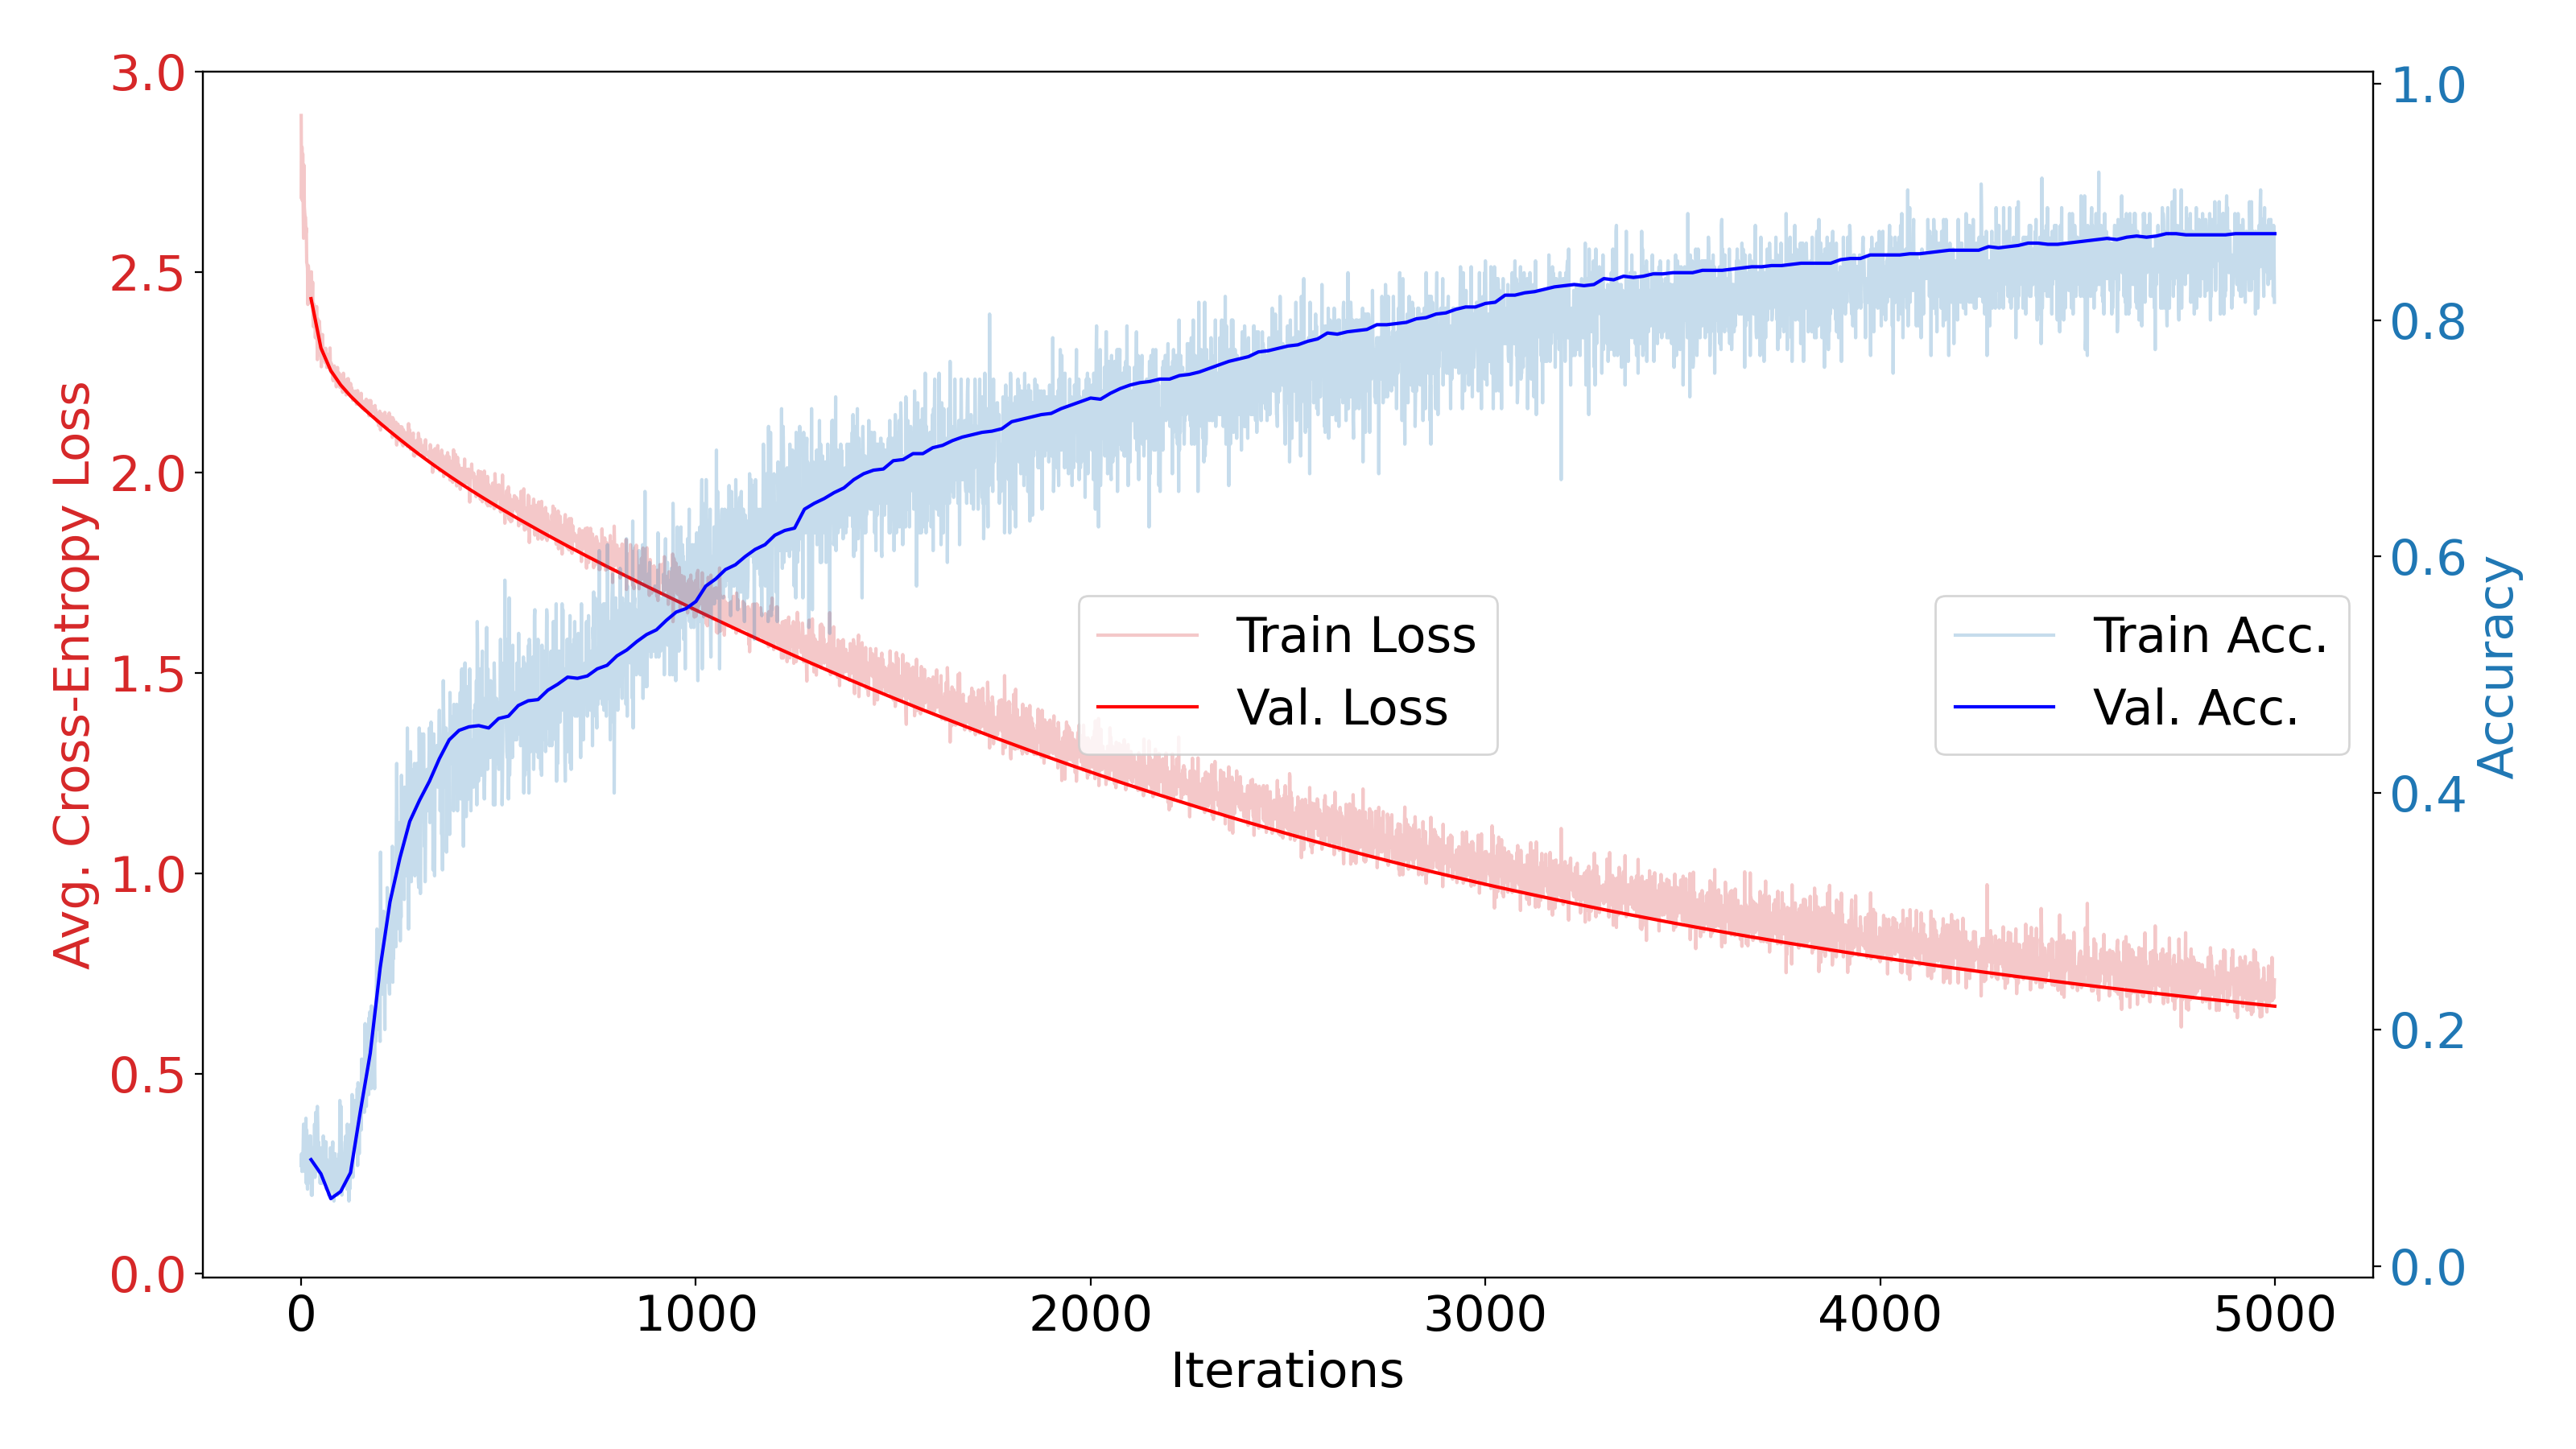
\includegraphics[width=.5\textwidth]{figures/1.png}
    \caption{Loss and accuracy over time}
\end{figure}
    \subsection*{Q4}
        The following are our plots for loss and accuracy given different step sizes:
            \begin{figure}[!htb]
                \minipage{0.32\textwidth}
                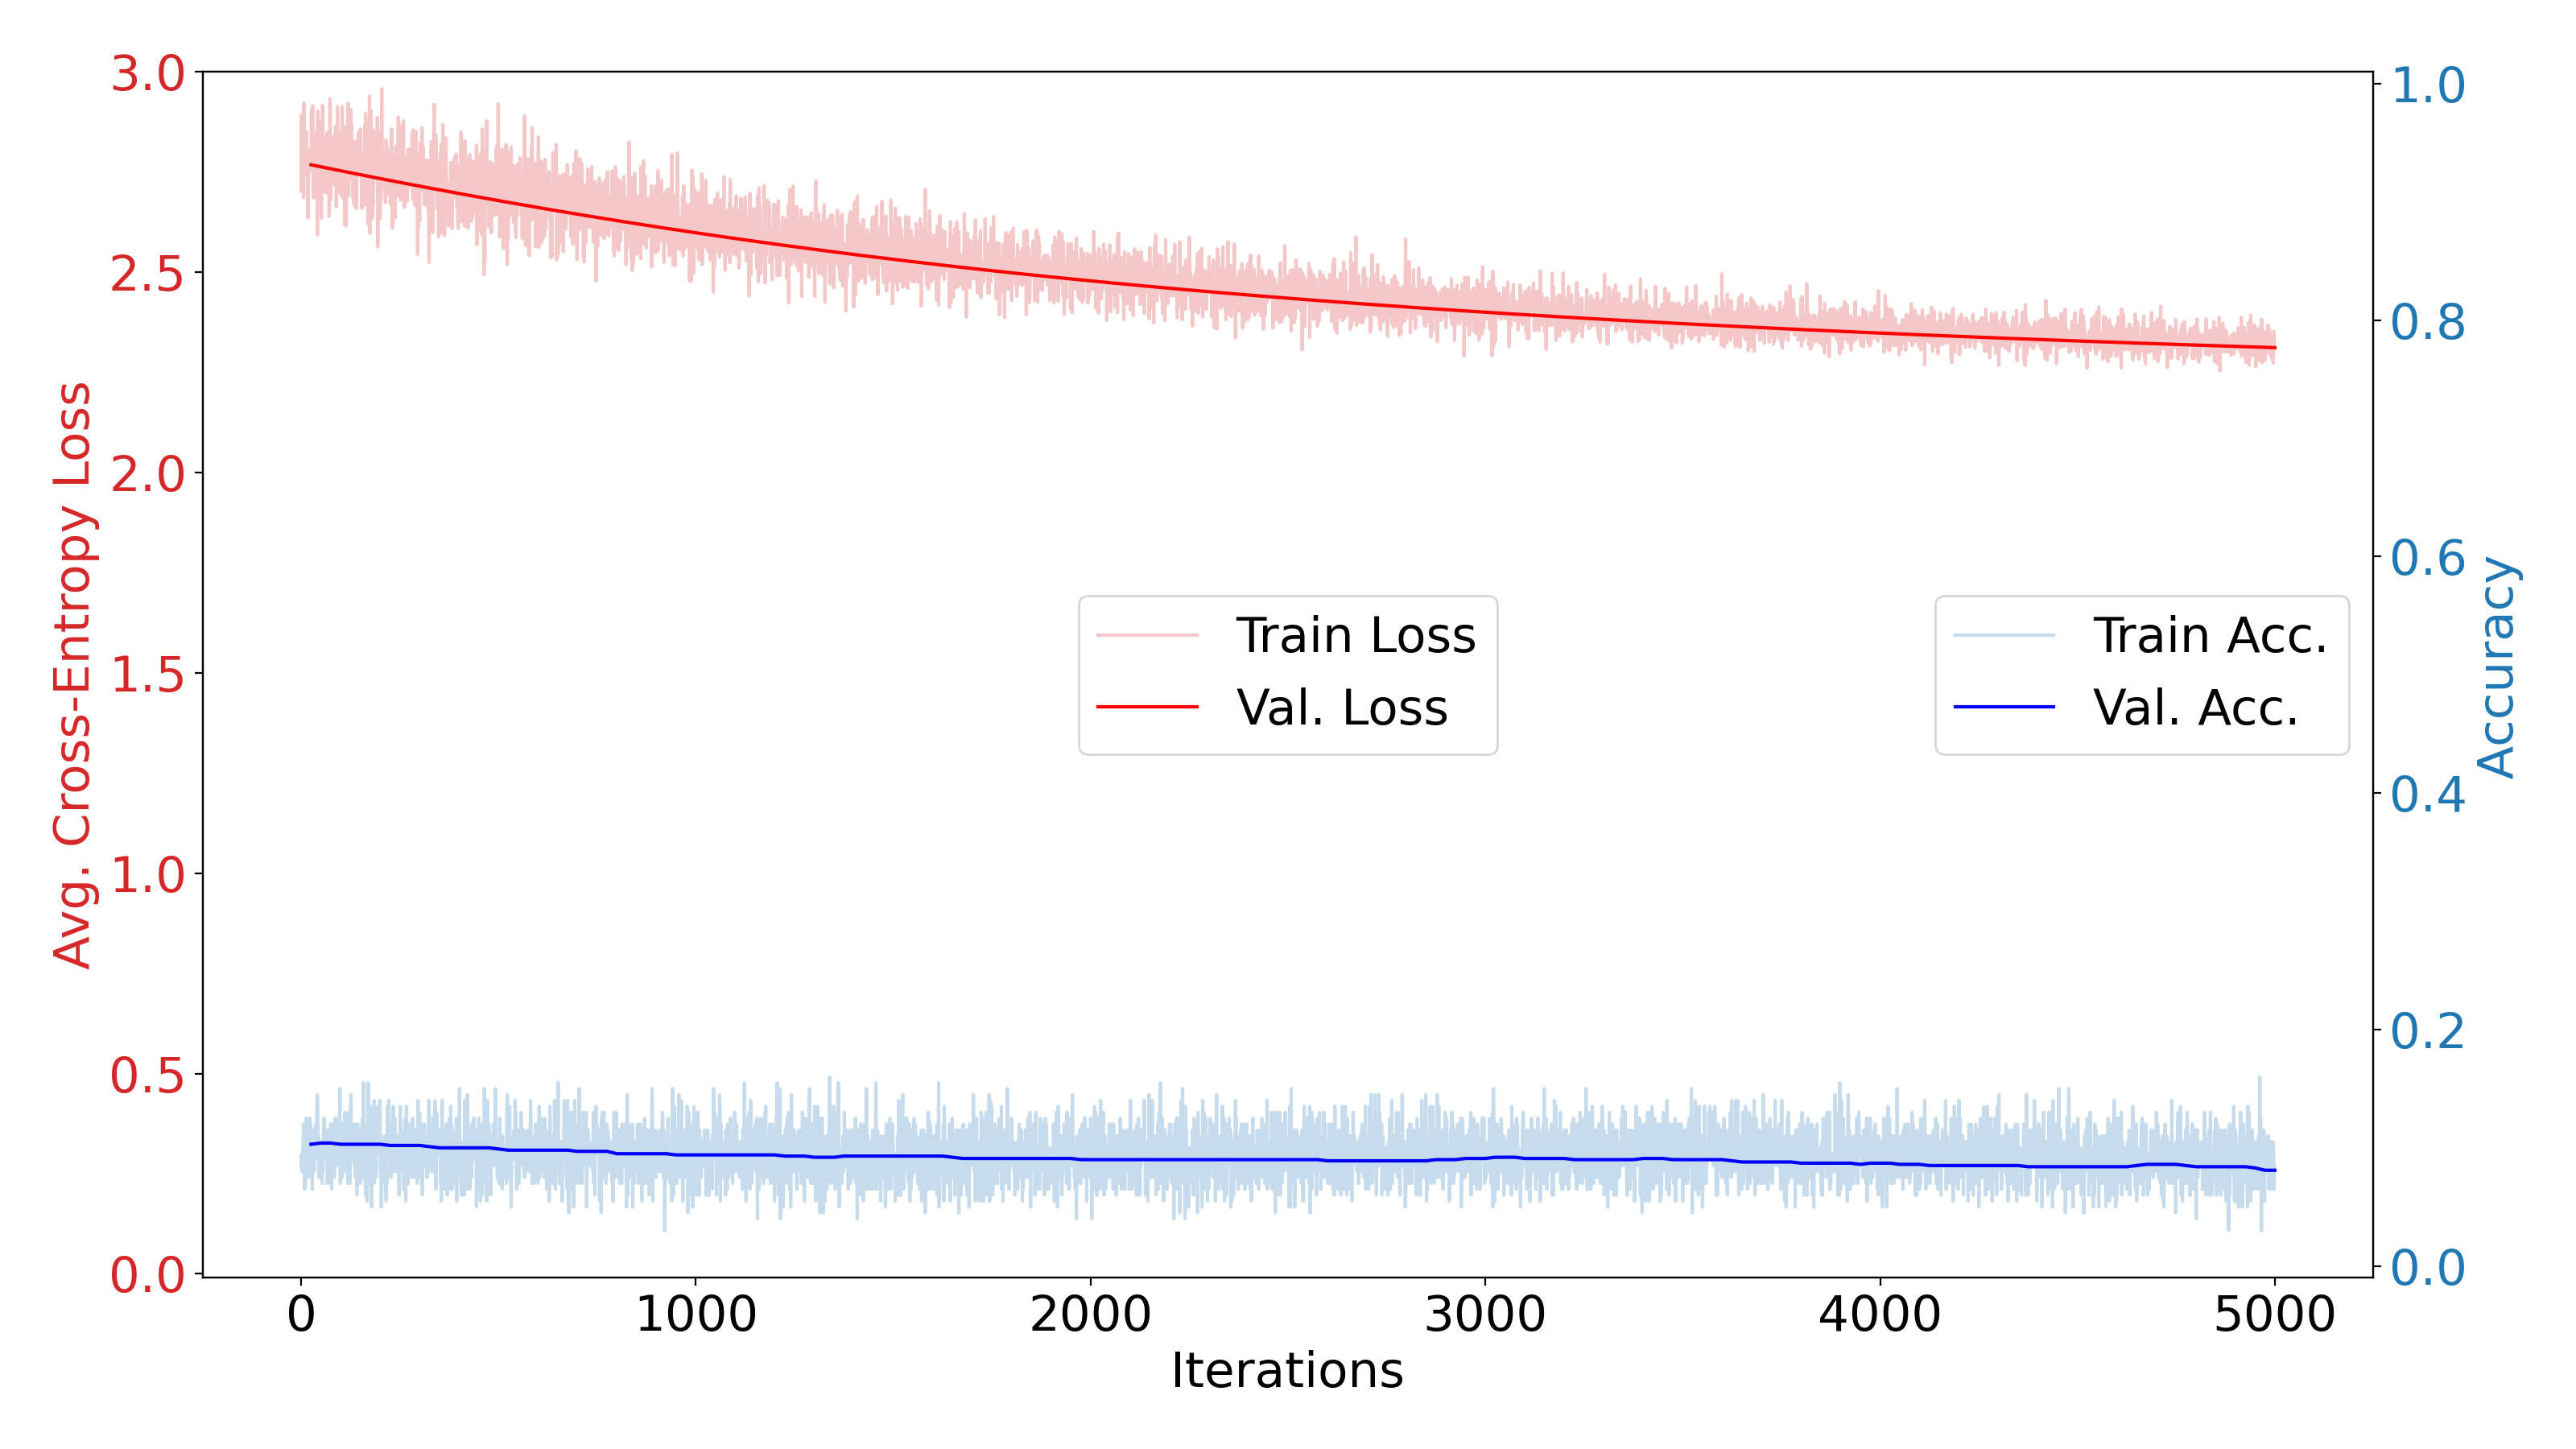
\includegraphics[width=\linewidth]{figures/2.png}
                \caption{step size $= 0.0001$}\label{fig:awesome_image1}
                \endminipage\hfill
                \minipage{0.32\textwidth}
                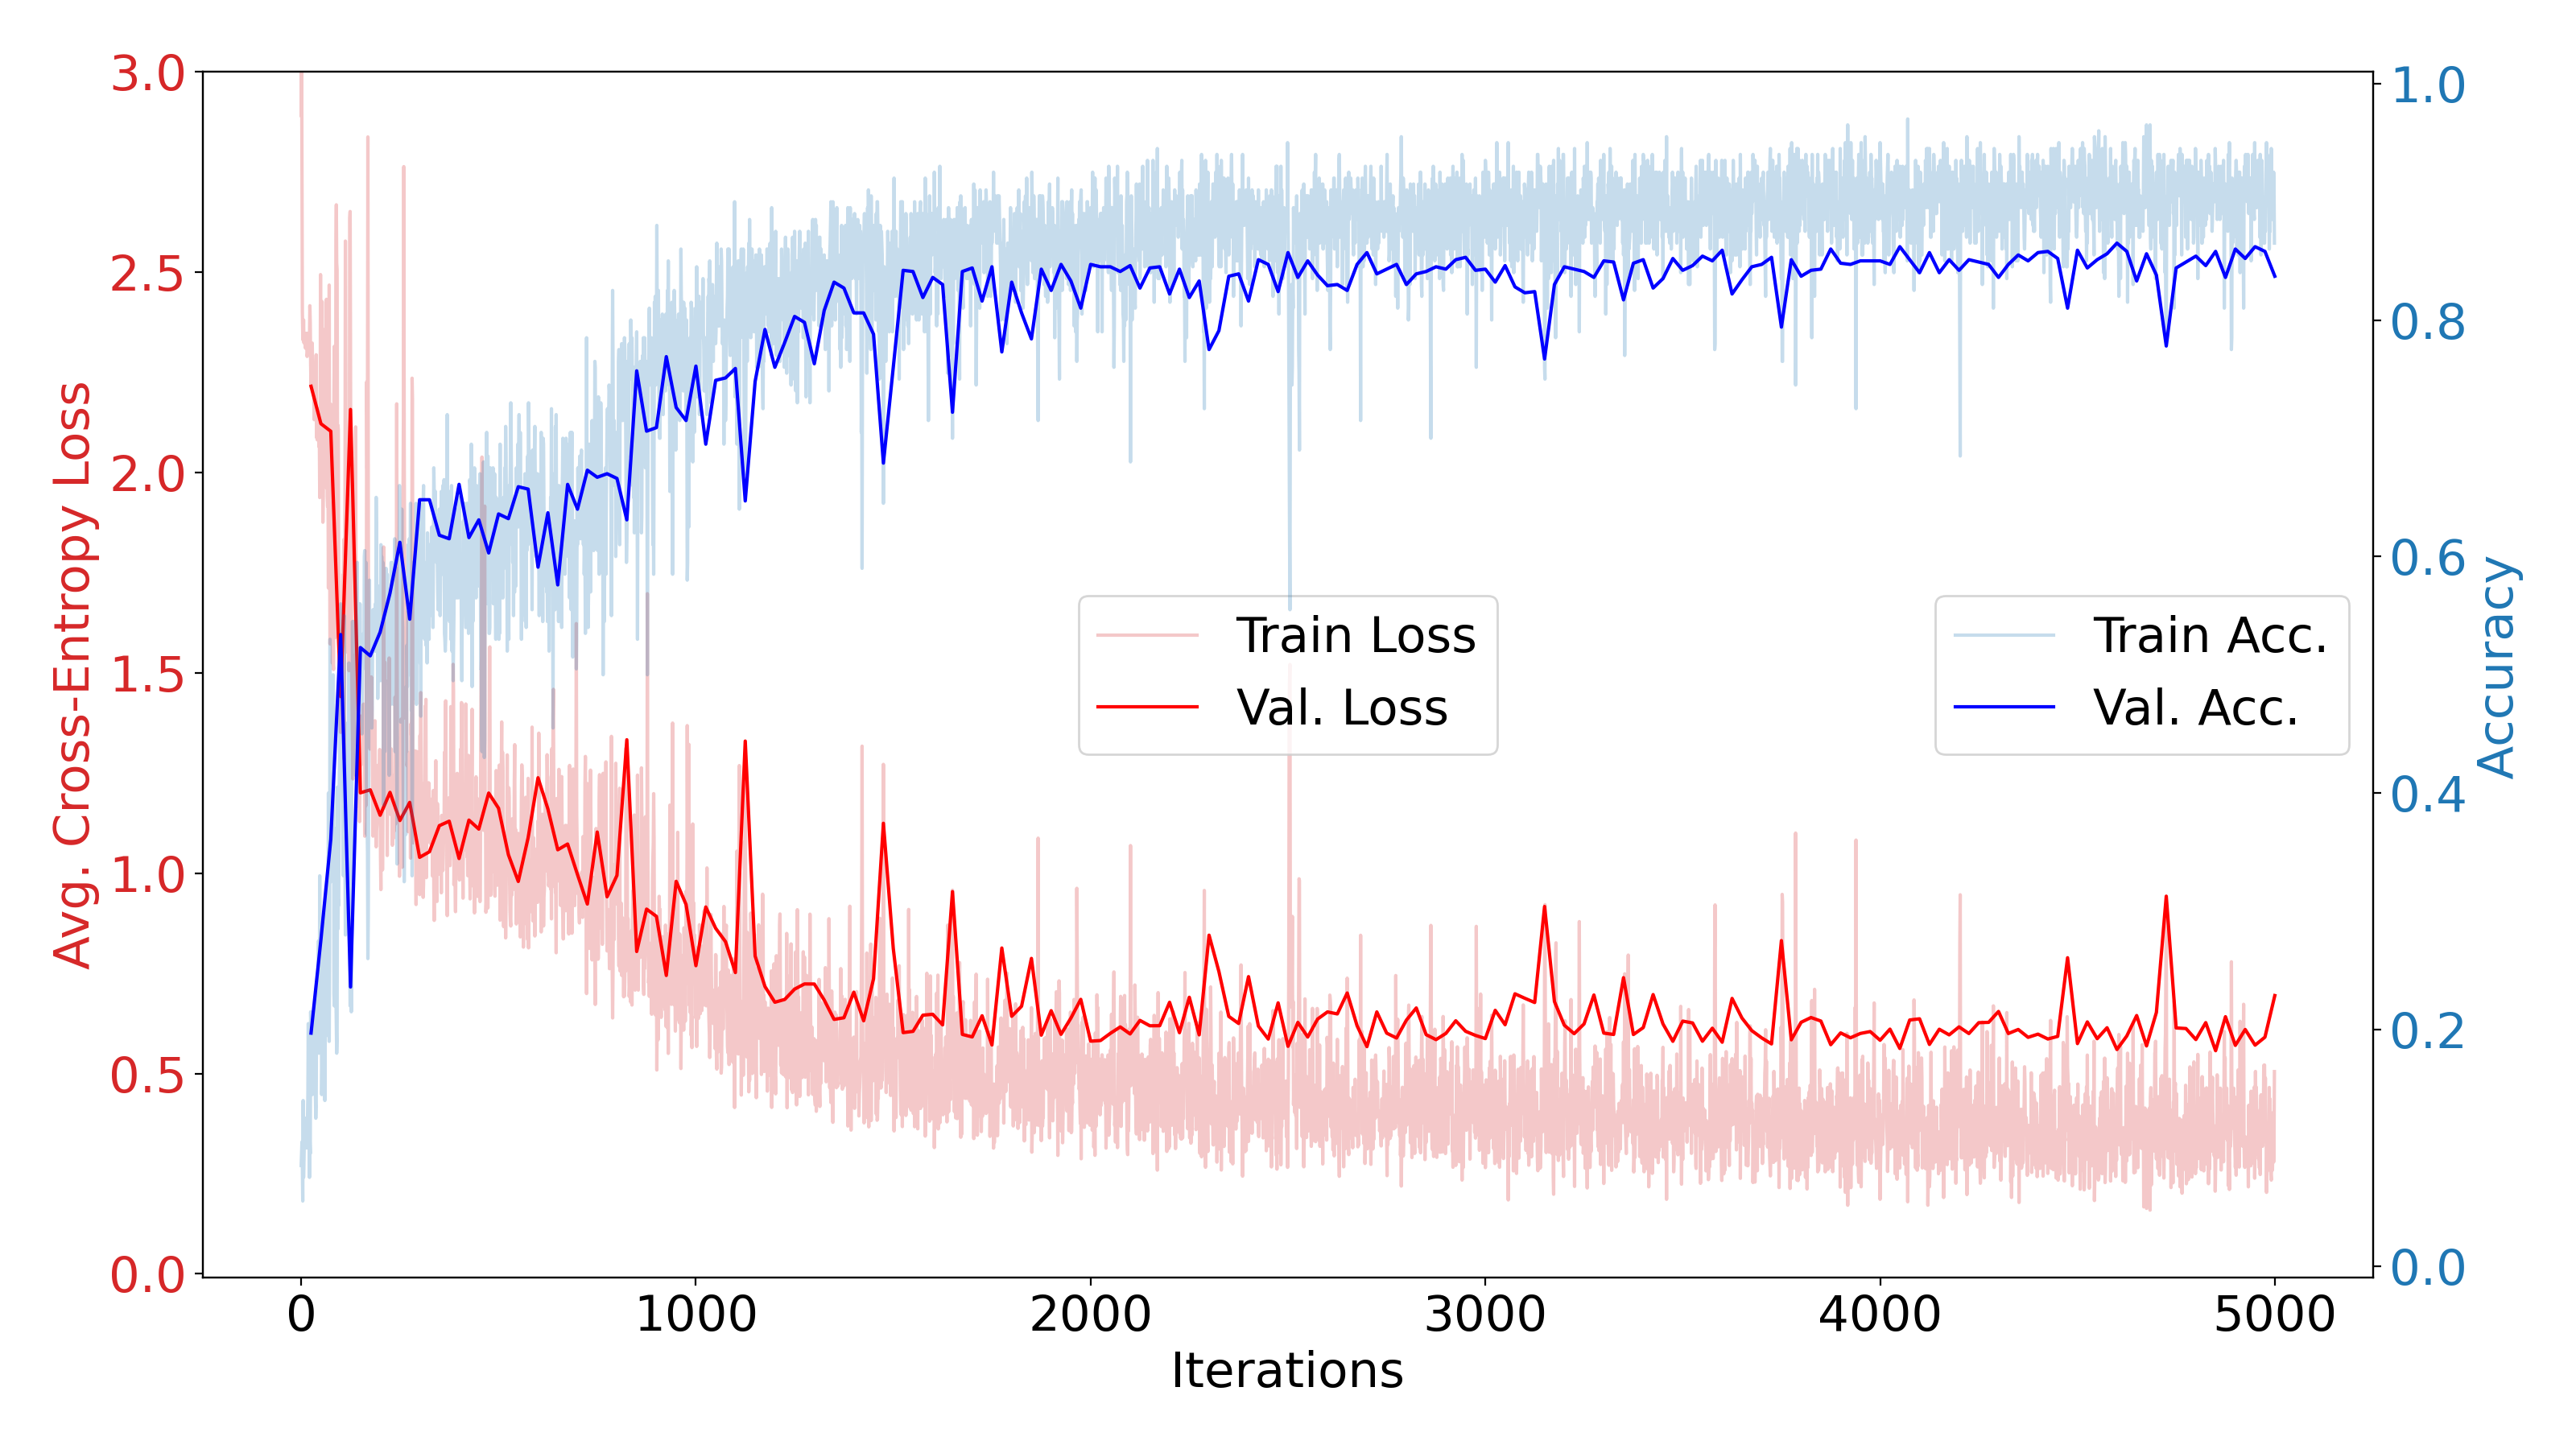
\includegraphics[width=\linewidth]{figures/3.png}
                \caption{step size $= 5$}\label{fig:awesome_image2}
                \endminipage\hfill
                \minipage{0.32\textwidth}%
                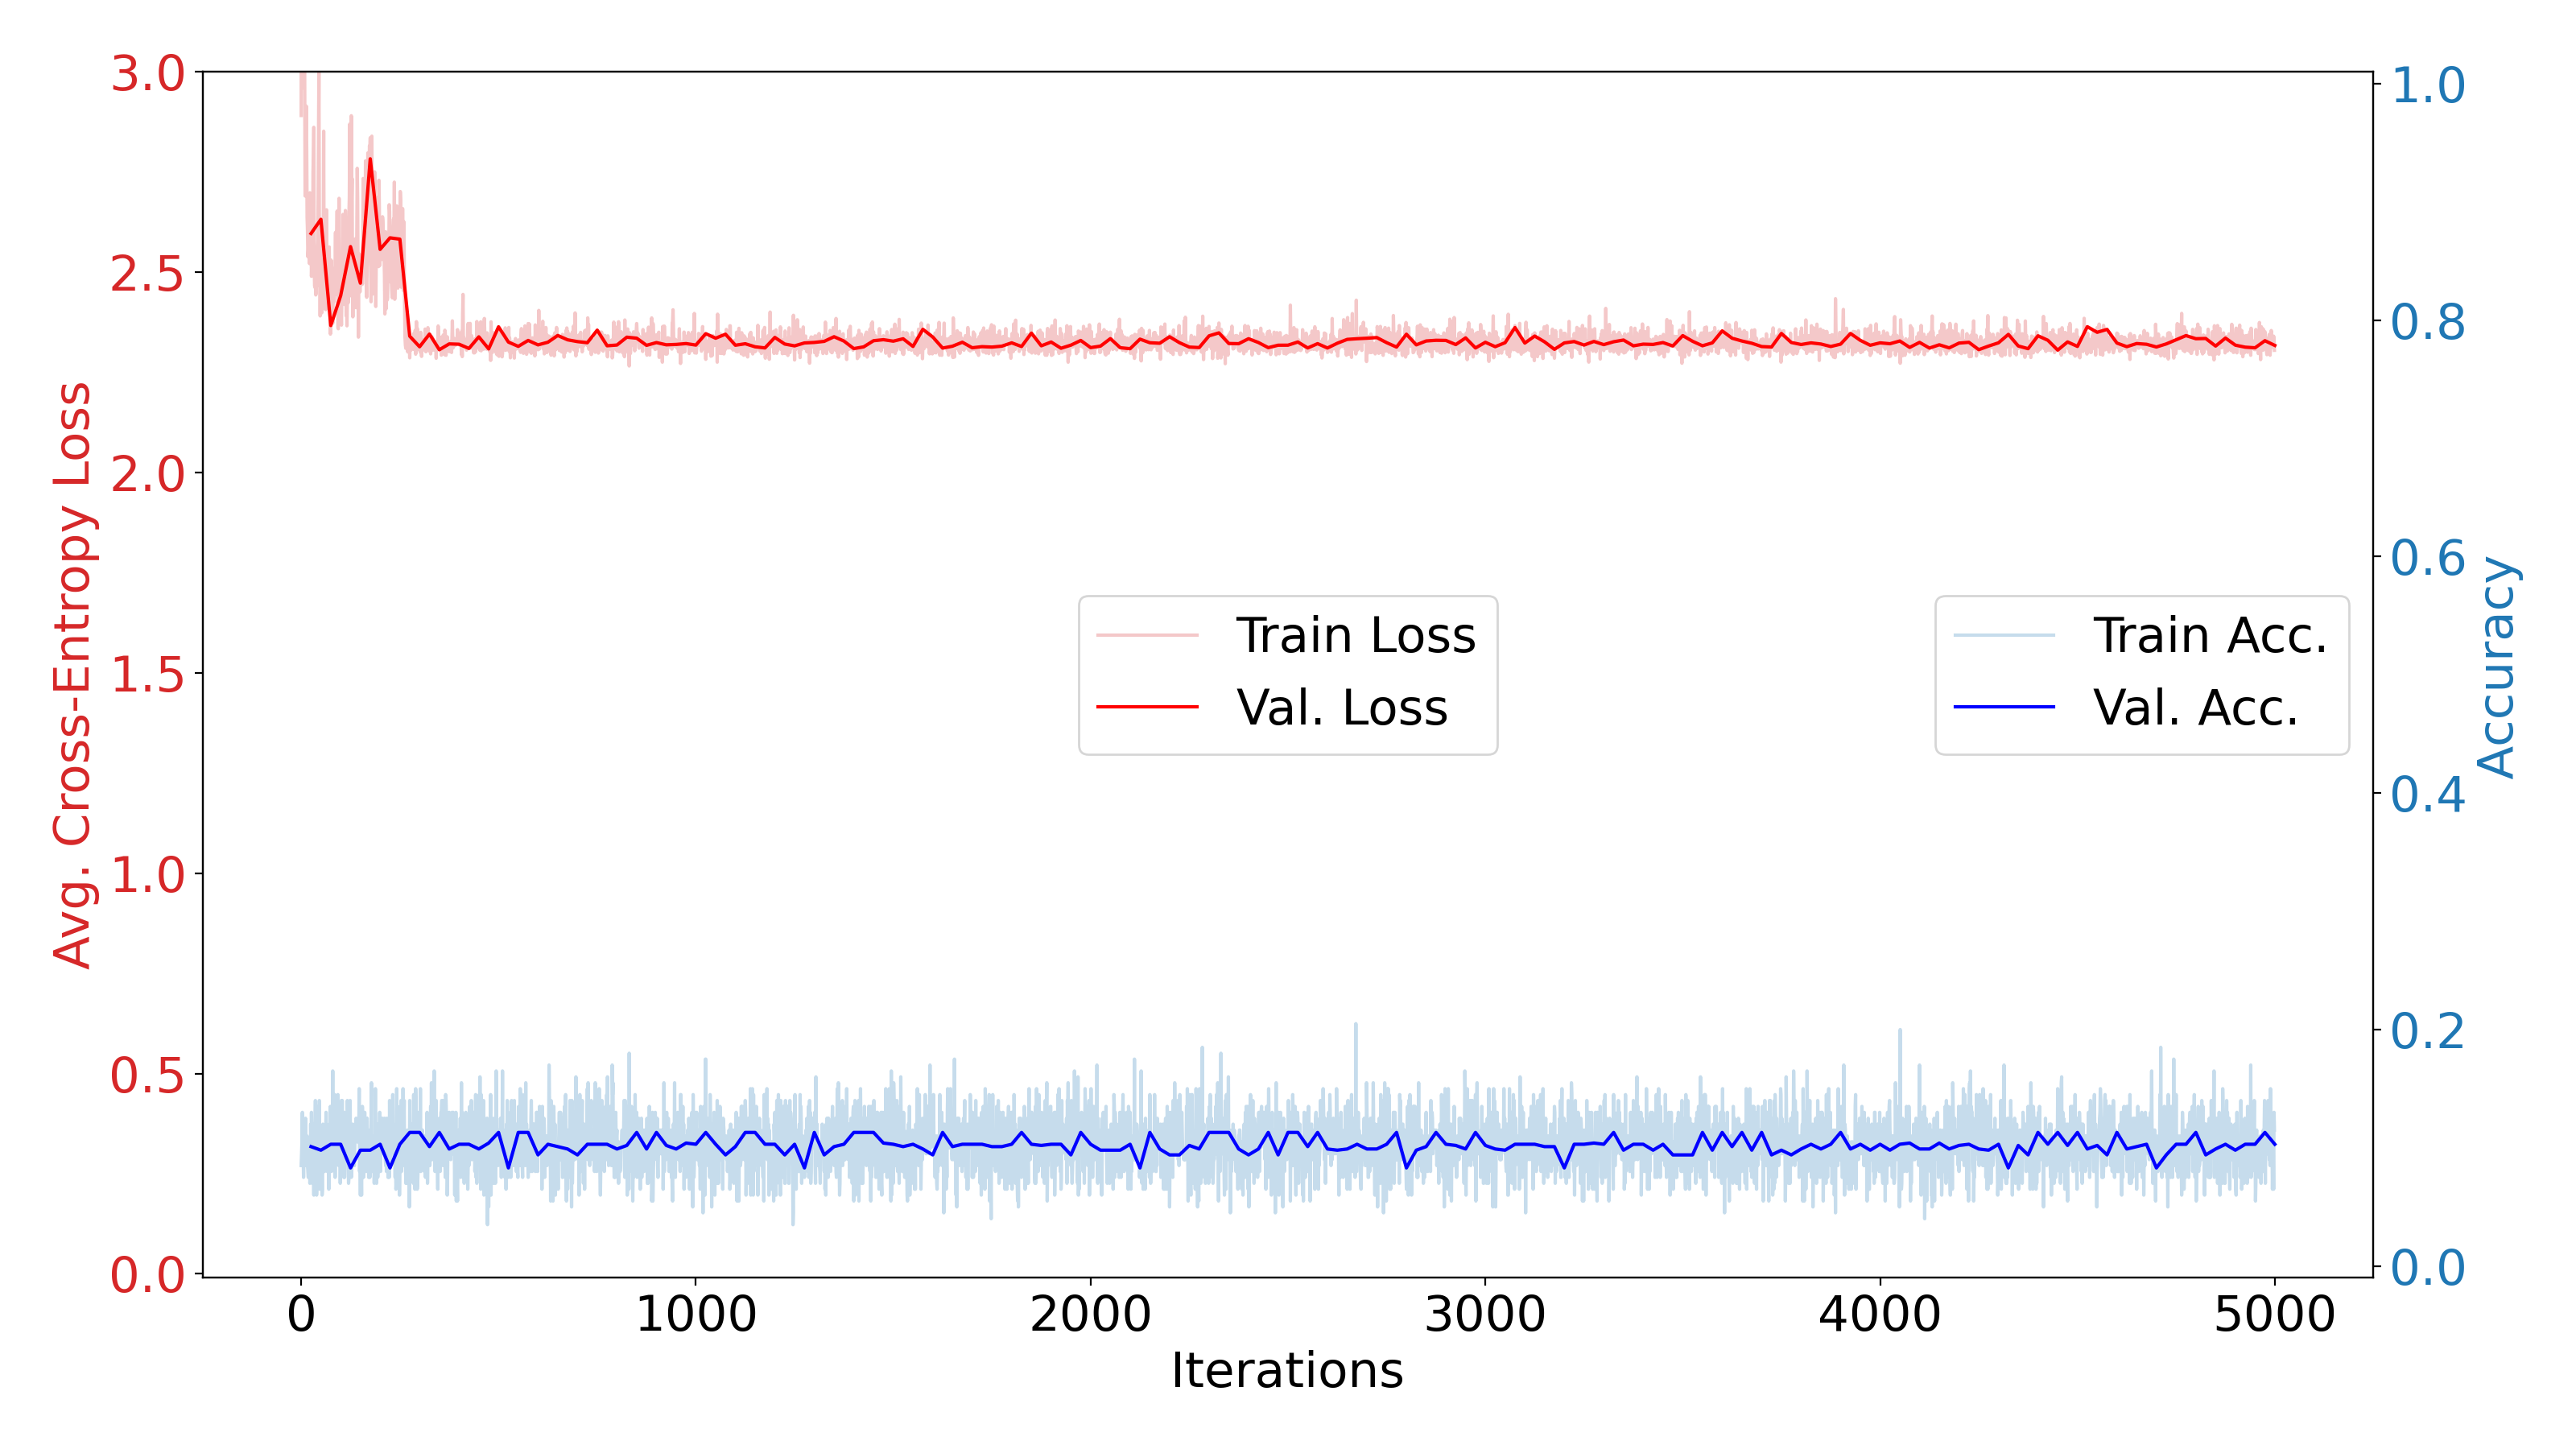
\includegraphics[width=\linewidth]{figures/4.png}
                \caption{step size $= 10$}\label{fig:awesome_image3}
                \endminipage
            \end{figure}
        \subsubsection*{a)}
            As we can see, \fbox{Figure 2} is quite smooth, but it takes too long to converge, 
            and we don't really see any increase in our accuracy. In \fbox{Figure 3}, we see that 
            the model does converge pretty quickly, but it also is overfitting fairly quickly, 
            and the entire graph is quite noisy. This means that we might get a model that is 
            much less accurate just by random chance of when we stop training the model.
            With \fbox{Figure 4} we see almost no motion and just noise. This is because our 
            step size is far too large. I would expect to see more noise as our model jumps around,
            but I suppose that this is not the case...
        \subsubsection*{b)}
            If the max epochs were increased, for a neural net with a step size of 0.0001 
            I would expect it to eventually look like \fbox{Figure 1} if given a sufficient number 
            of iterations. However, it may be the case that we get stuck in some very small local 
            minimum due to the tininess of our step size.
    \subsection*{Q5}
        The plots for our variations in hyperparameters are given in \fbox{Figure 5}, \fbox{Figure 6}, \fbox{Figure 7}.
            \begin{figure}[!htb]
                \minipage{0.32\textwidth}
                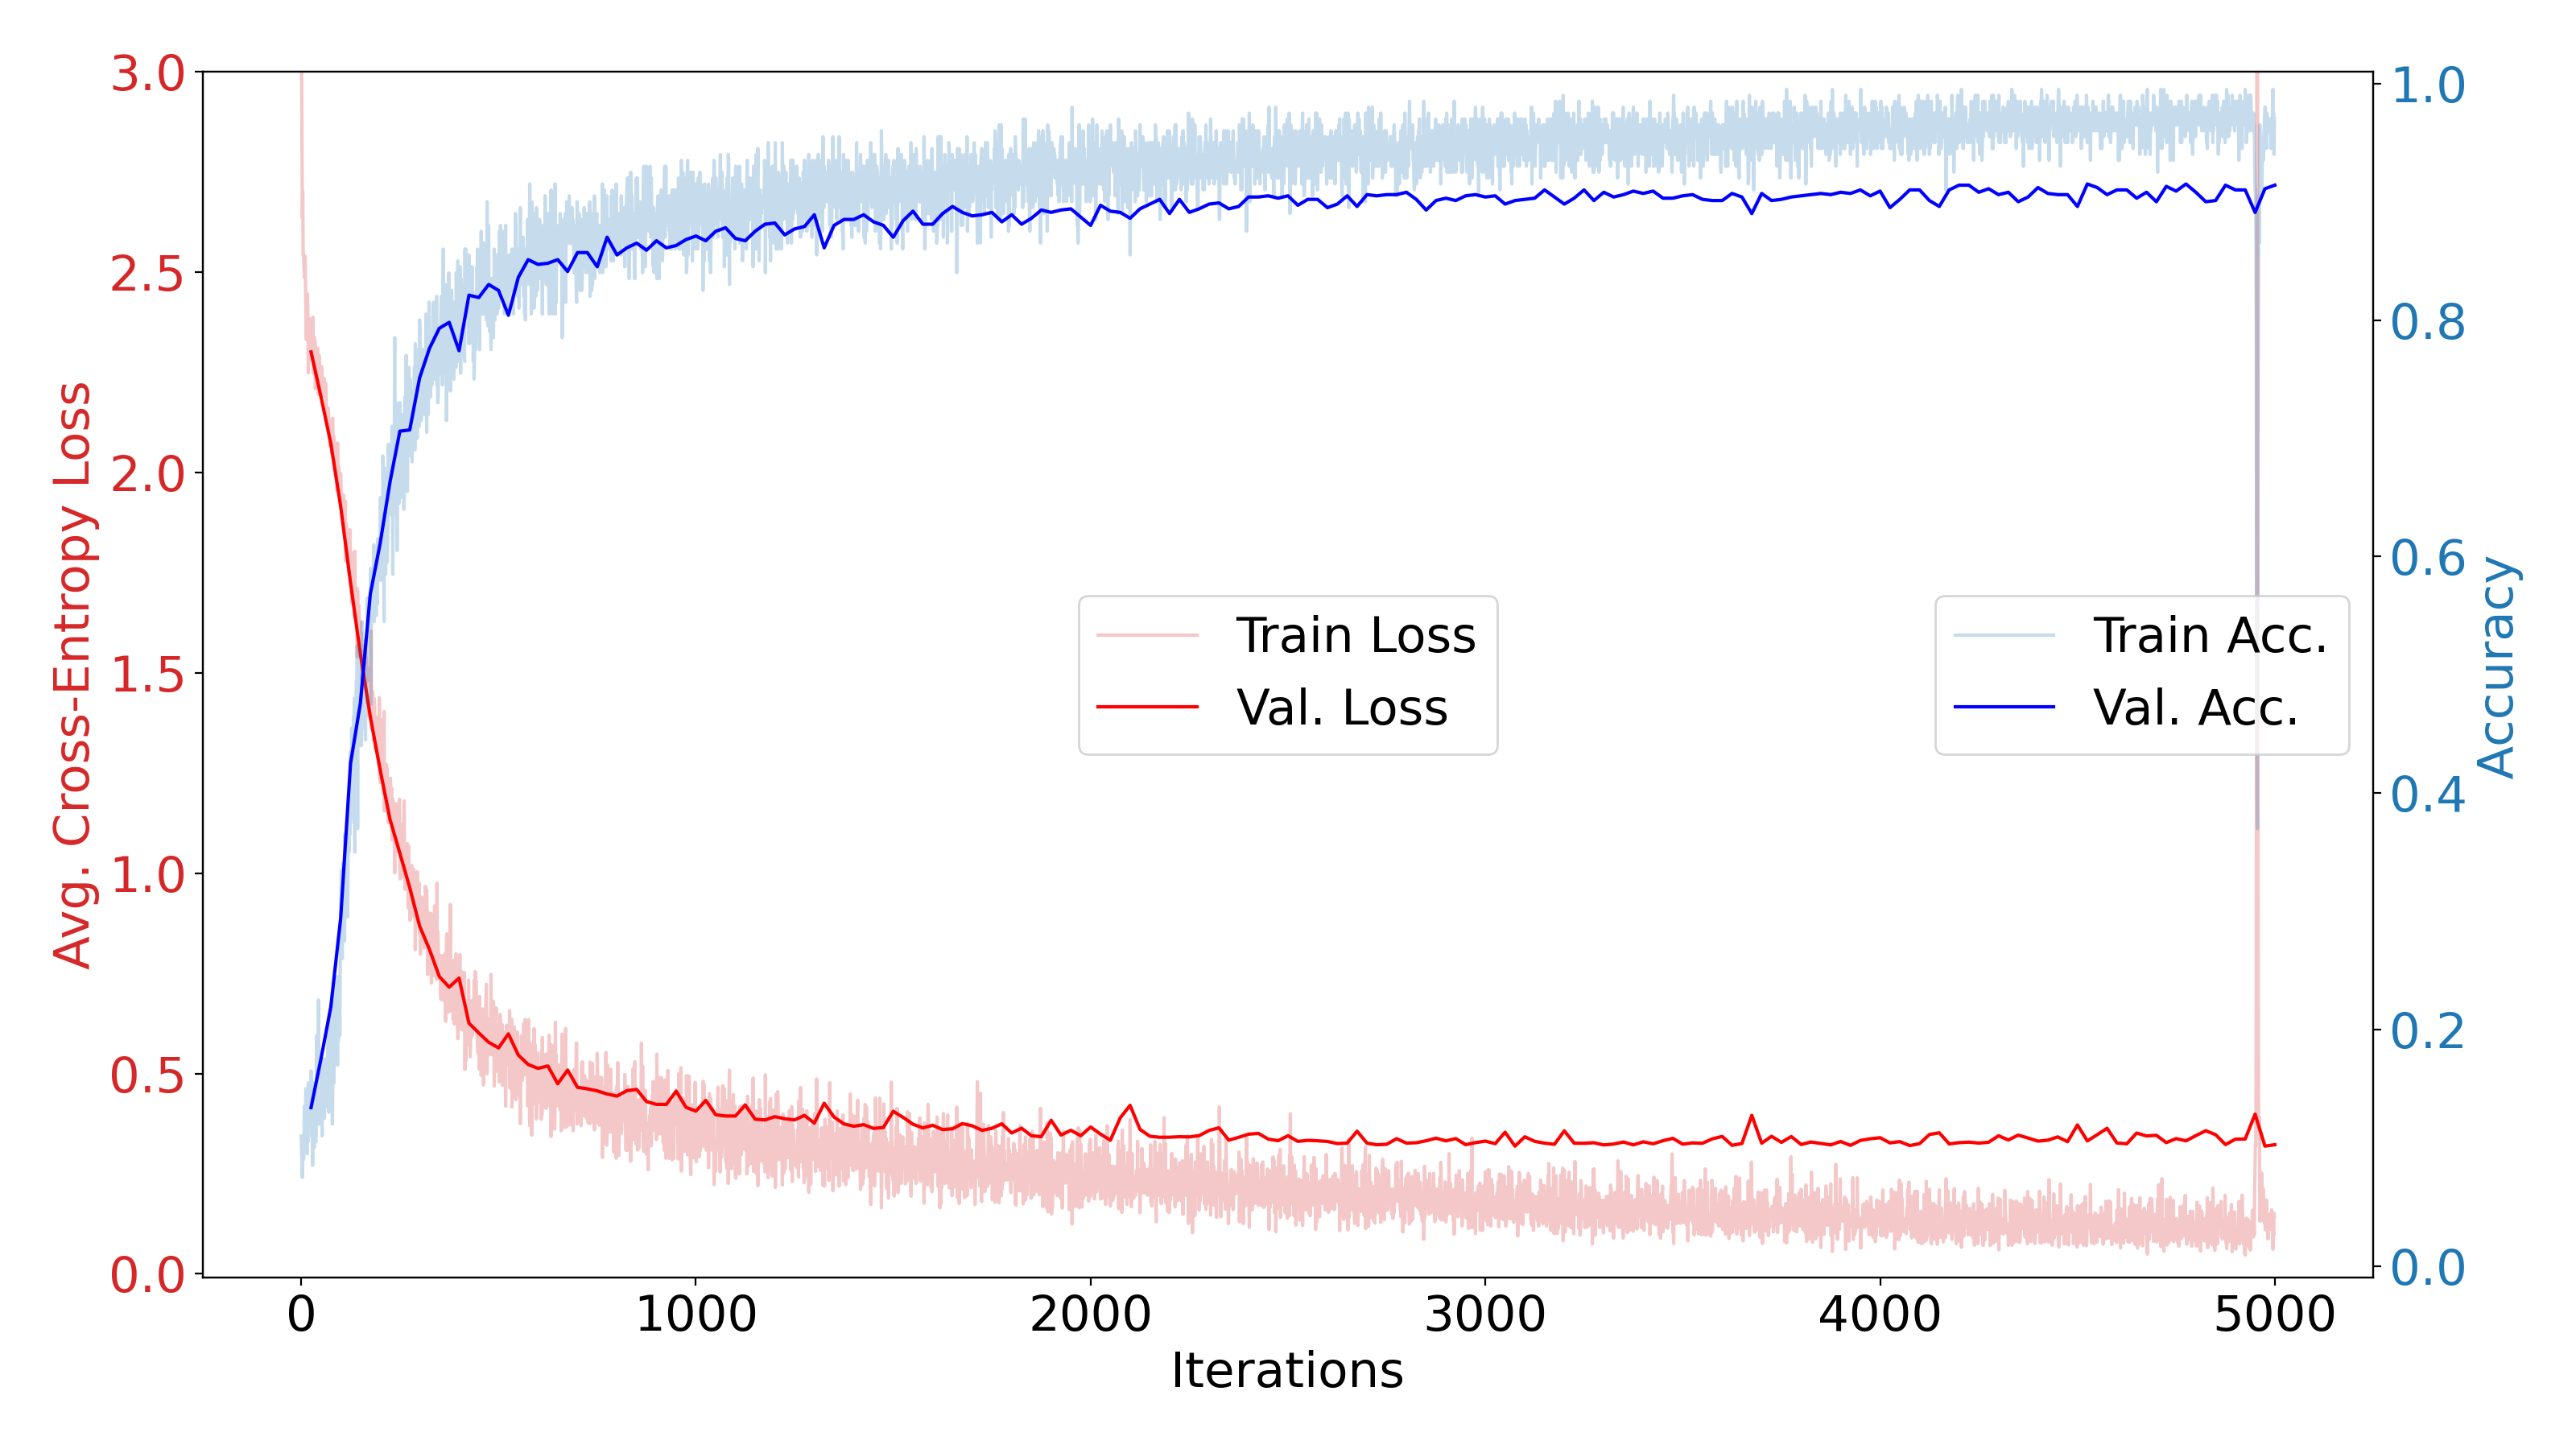
\includegraphics[width=\linewidth]{figures/5_1.png}
                \caption{5-layer with Sigmoid Activation}\label{fig:awesome_image1}
                \endminipage\hfill
                \minipage{0.32\textwidth}
                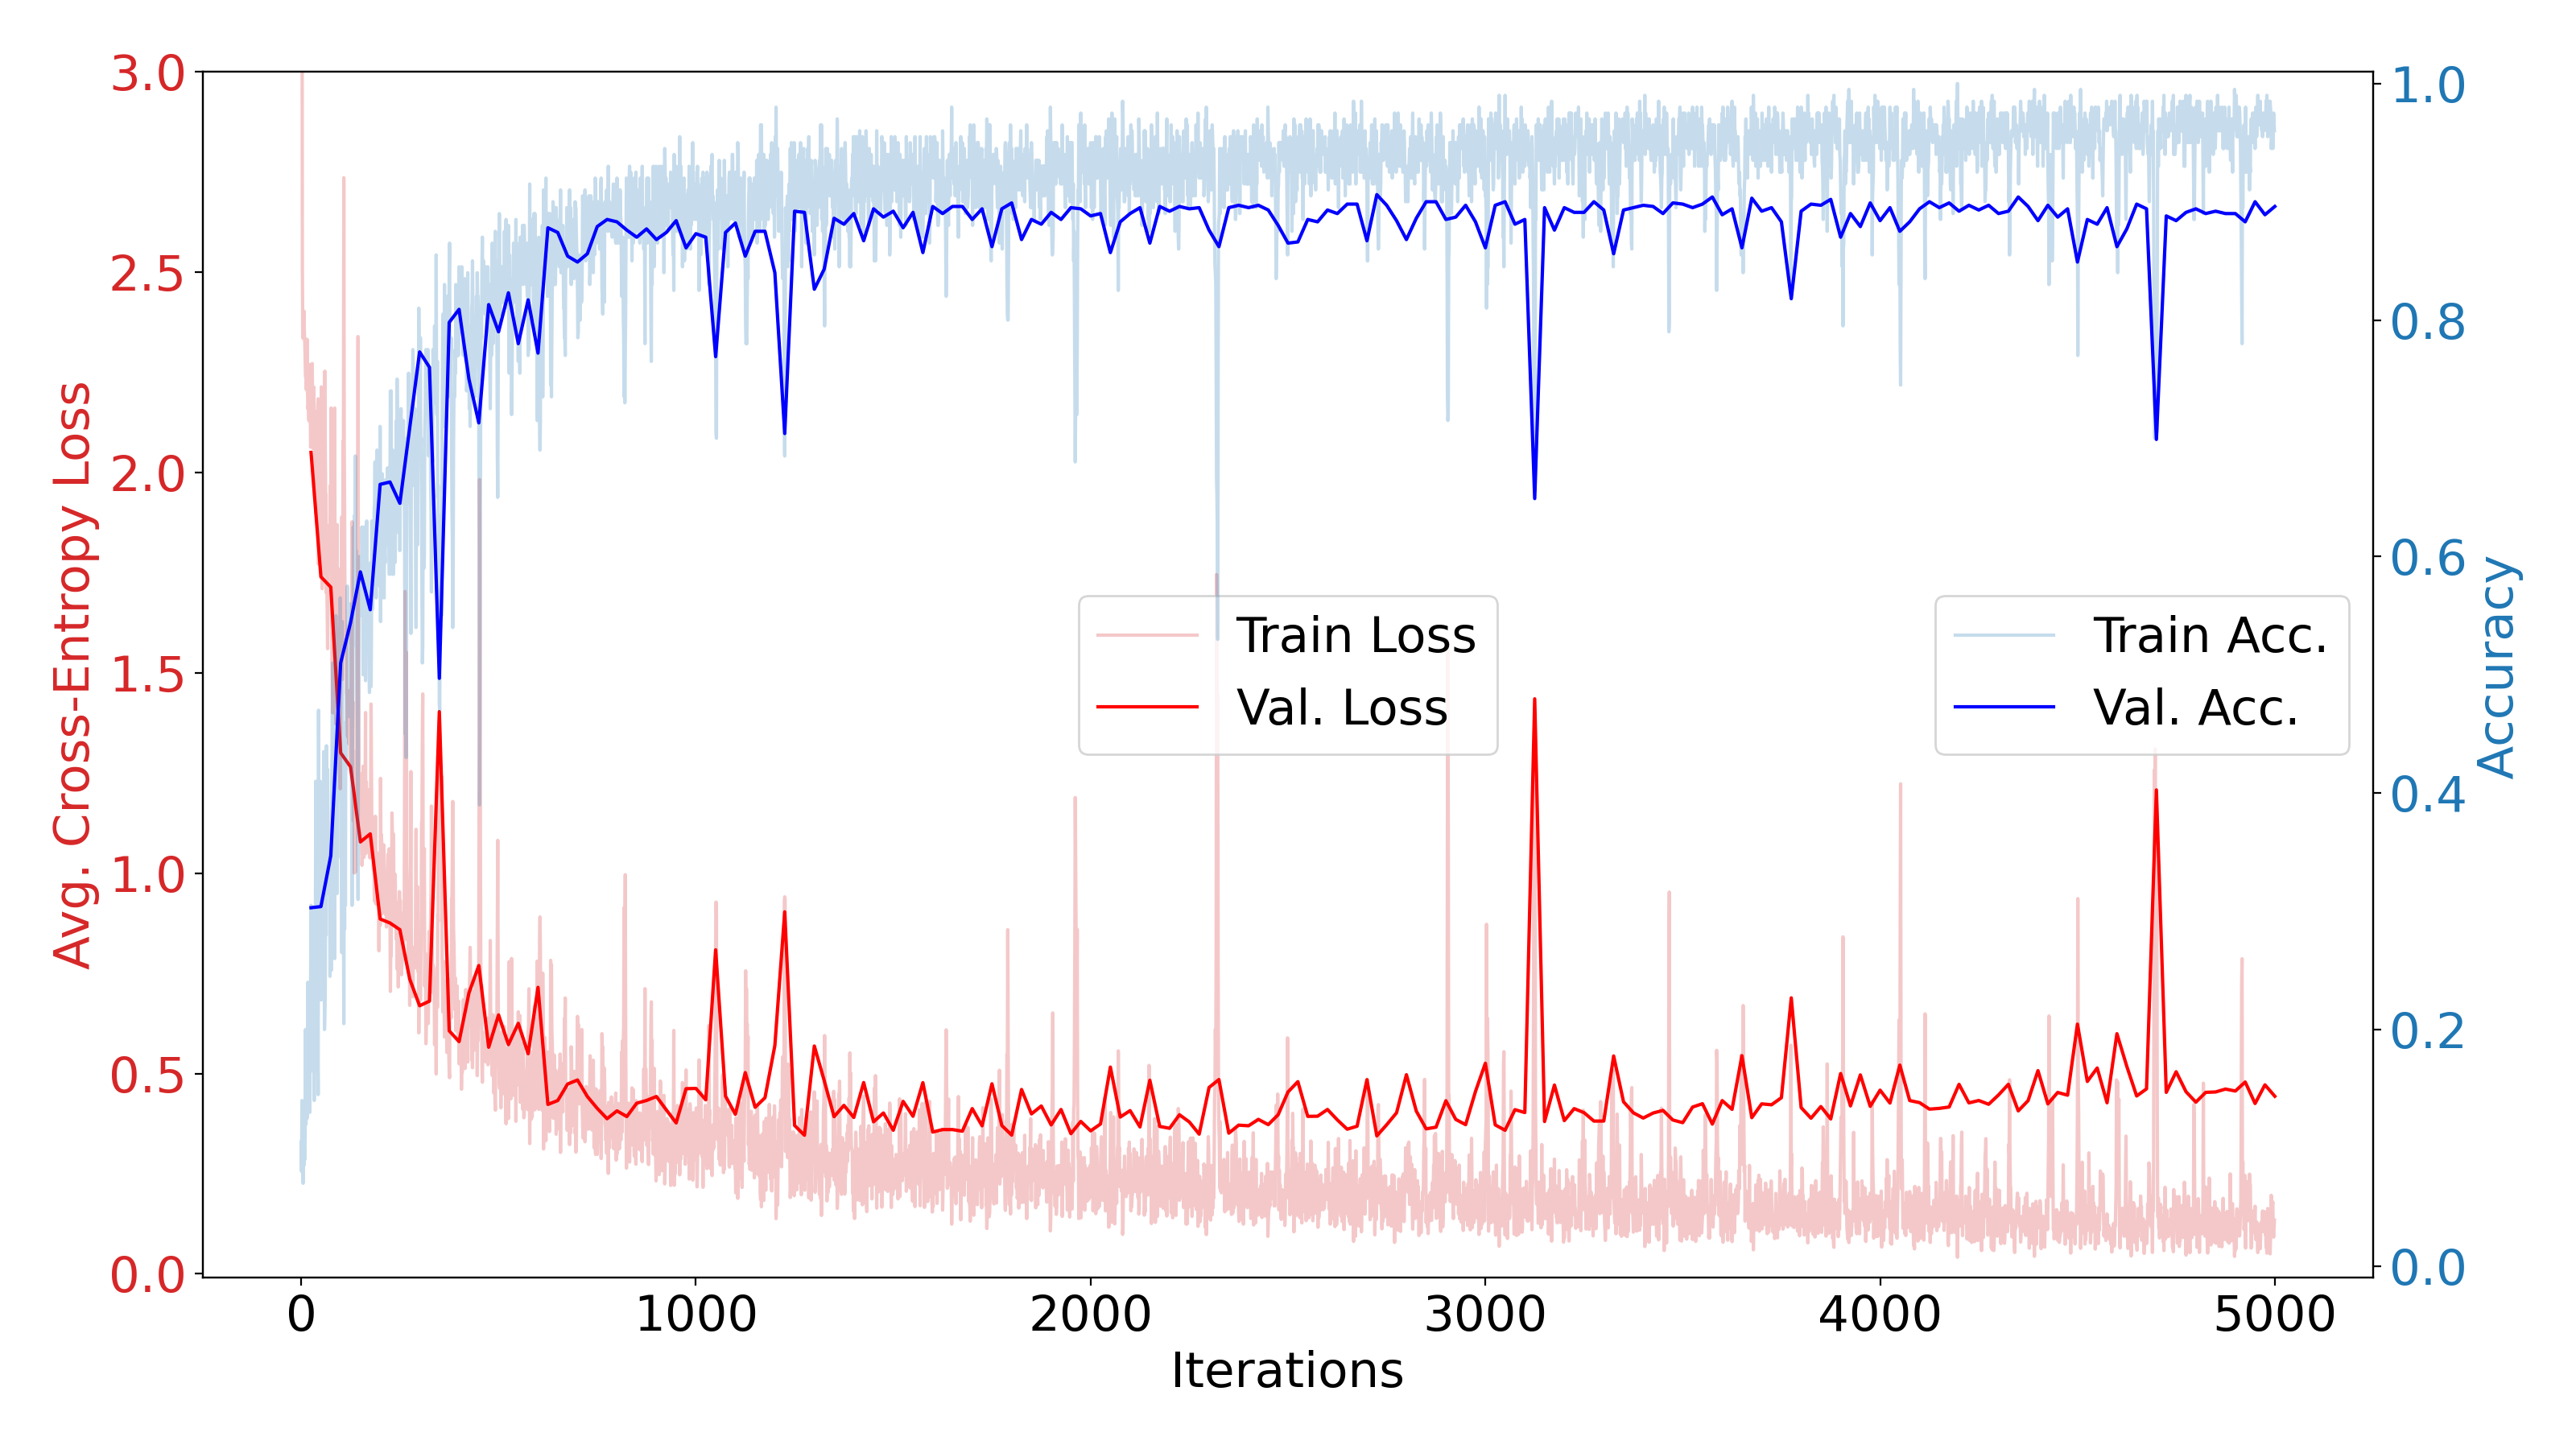
\includegraphics[width=\linewidth]{figures/5_2.png}
                \caption{5-layer with Sigmoid Activation with 0.1 step size}\label{fig:awesome_image2}
                \endminipage\hfill
                \minipage{0.32\textwidth}%
                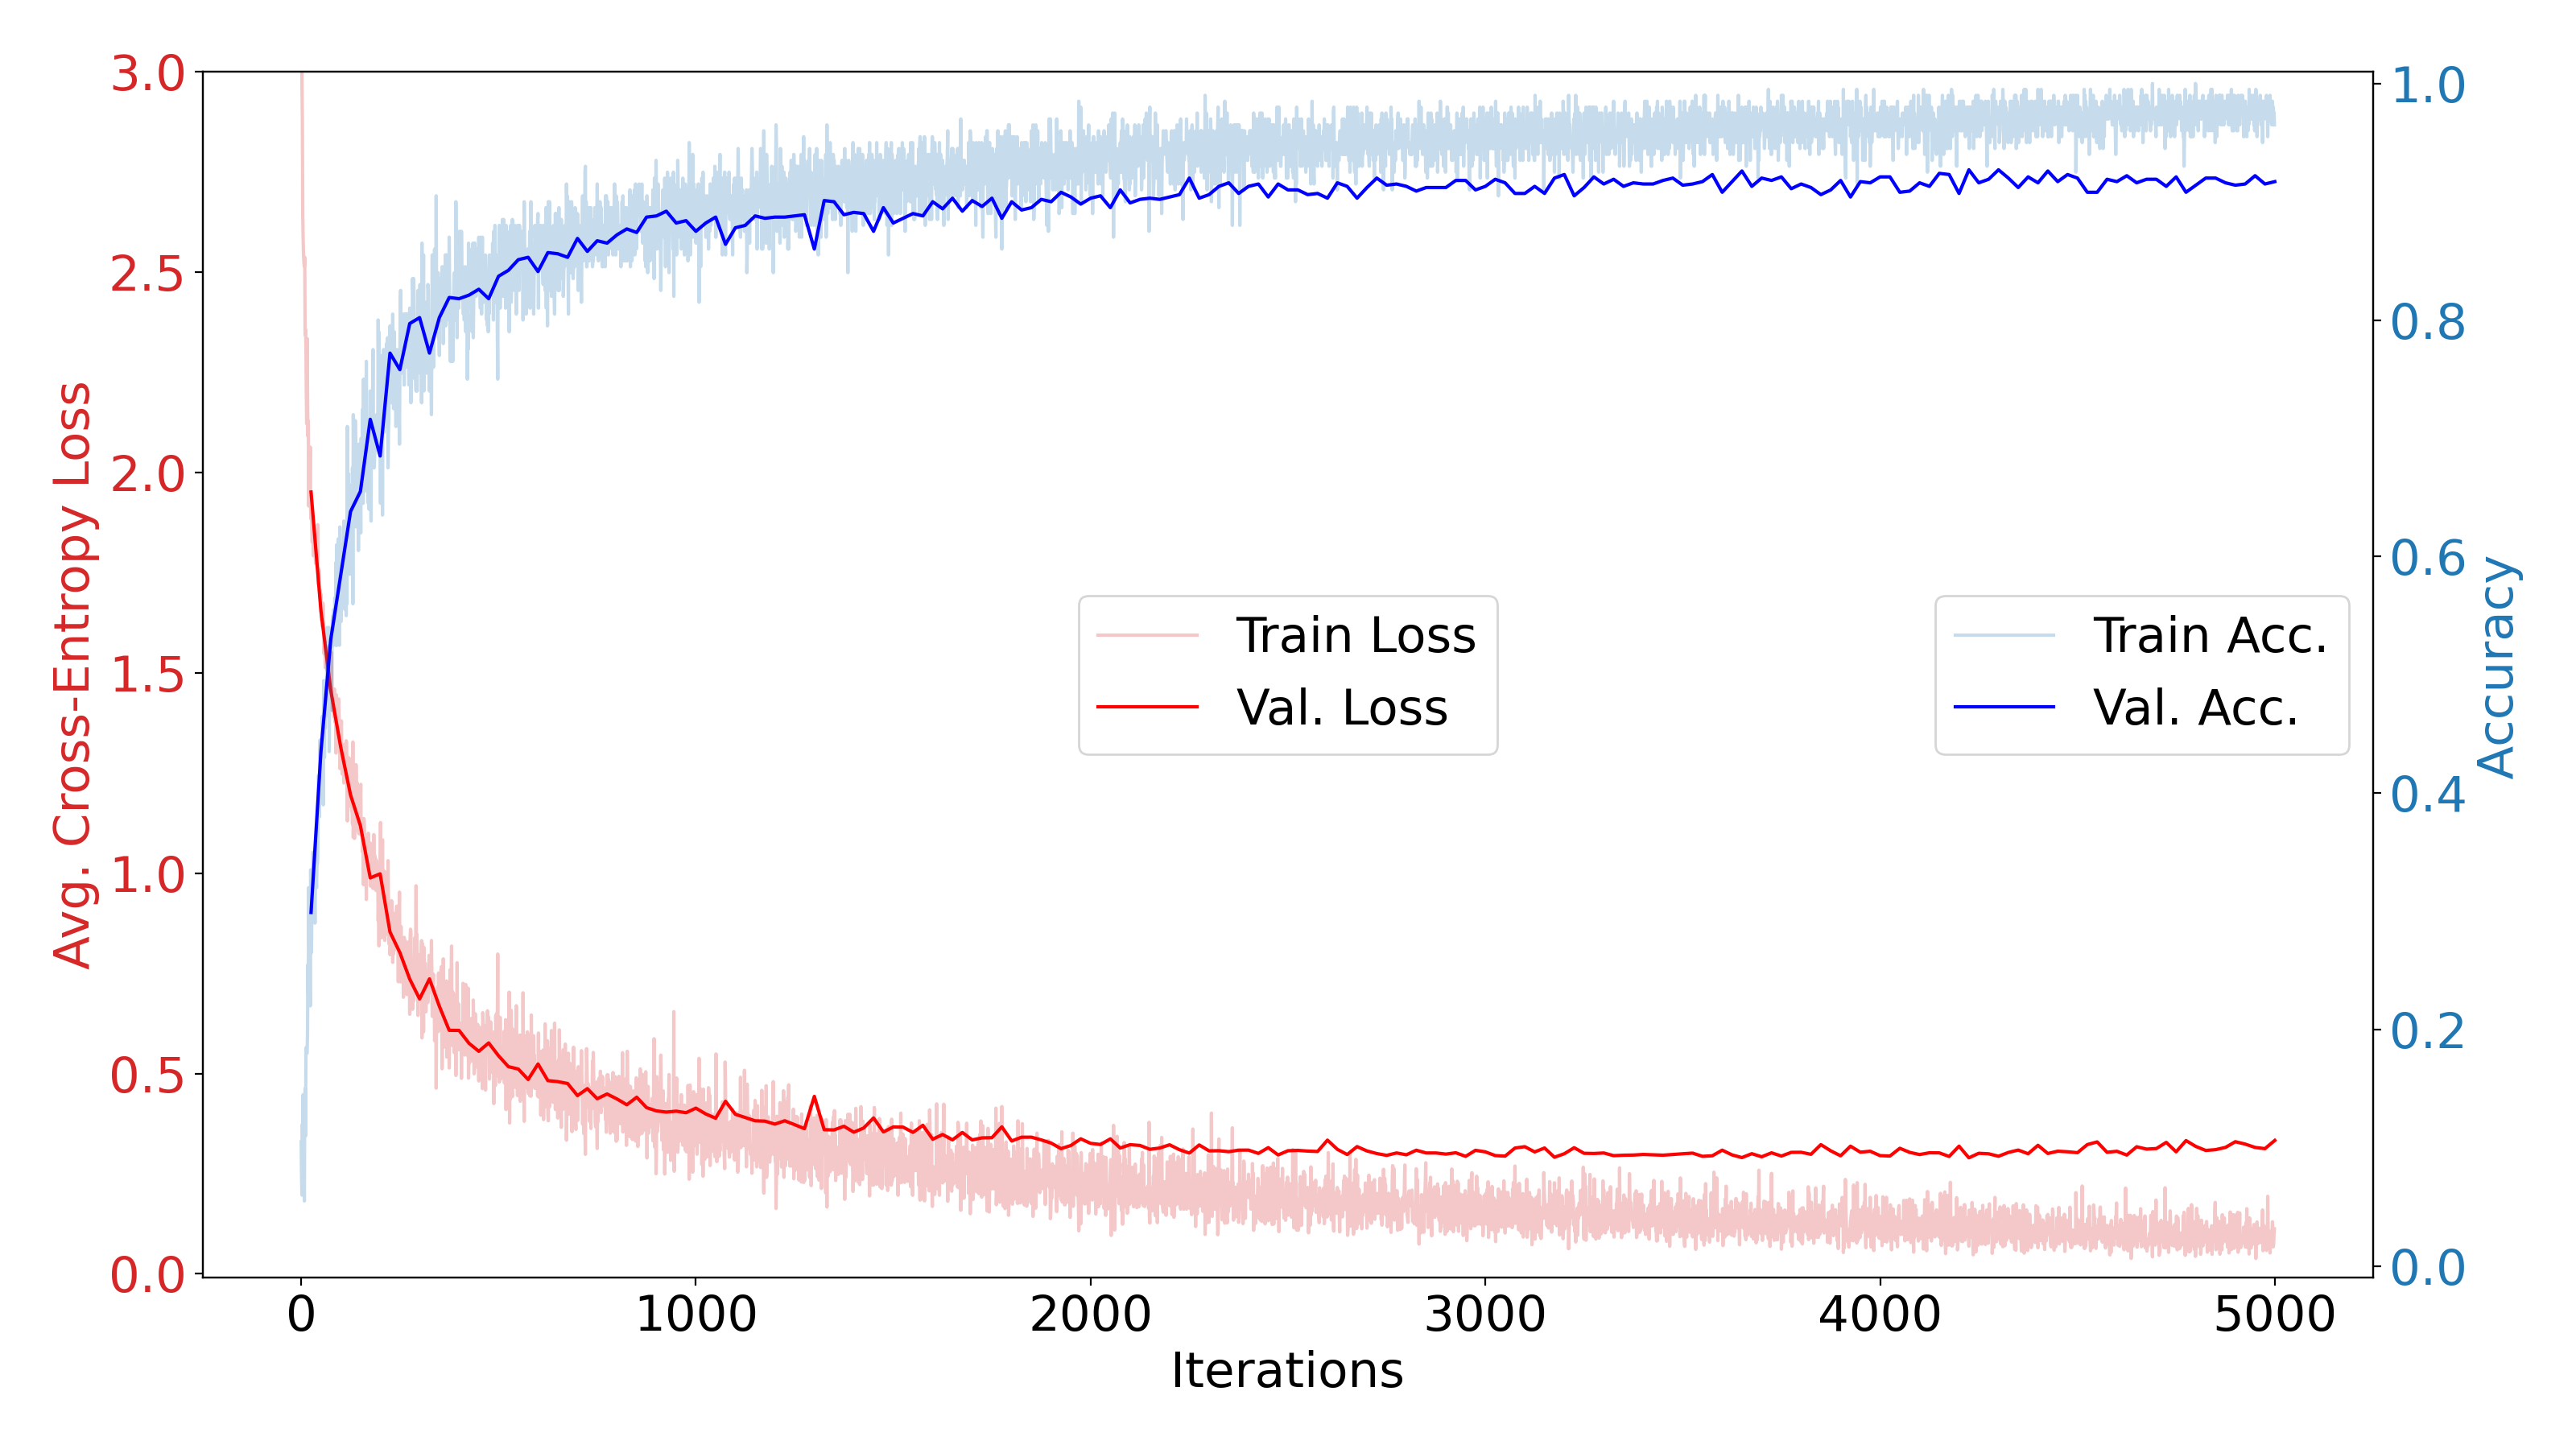
\includegraphics[width=\linewidth]{figures/5_3.png}
                \caption{5-layer with ReLU Activation}\label{fig:awesome_image3}
                \endminipage
            \end{figure}
        \subsubsection*{a)}
            In \fbox{Figure 5} we can see that we increase performance on the training data over time,
            but the performance on validation seems to stop improving about a third of the way through.
            The shape of all 3 is very similar. However, whith a larger step size in \fbox{Figure 6} we 
            see that the graph is much less smooth. In all three, the performance on the training data 
            goes well beyond the validation performance.
        \subsubsection*{b)}
            There does not seem to be an increased learning rate, and this may be because even though the 
            step size is larger, the amount of mistakes/backtracking that must occur also happens to balance
            out its faster nature.
        \subsubsection*{c)}
            One reason that reLU might outperform sigmoid may be that the gradient for a point that is very likely 
            to be classified as 0 or 1 will be steeper for reLU than for sigmoid, causing it to converge 
            more quickly on whatever model it may find.
    \subsection*{Q6}
We take 5 random seeds, and see variations in final accuracies.
\begin{verbatim}
    Loss:    0.6744     Train Acc:     86.42%      Val Acc:      89.1%
    Loss:     0.666     Train Acc:     87.06%      Val Acc:      88.5%
    Loss:     0.712     Train Acc:     86.06%      Val Acc:      87.7%
    Loss:    0.7025     Train Acc:     86.54%      Val Acc:      87.9%
    Loss:    0.6572     Train Acc:     86.32%      Val Acc:      87.4%
\end{verbatim}
The accuracies seemed to all remain within about $\pm 1$ of each other 
which makes me feel with some confidence that everything from before is fairly accurate.
Of course, the stochastic element of our gradient descent does effect the 
deterministic element of our machine learning model. However, since we must 
deal with bayes error regardless, this is probably fine.
    \subsection*{Q7}
    For the final submission I made, I used the following hyperparameters:
    \begin{verbatim}
# GLOBAL PARAMETERS FOR STOCHASTIC GRADIENT DESCENT
np.random.seed(102)
step_size = .001
batch_size = 200
max_epochs = 400

# GLOBAL PARAMETERS FOR NETWORK ARCHITECTURE
number_of_layers = 4
width_of_layers = 66  # only matters if number of layers > 1
activation = "ReLU" if False else "Sigmoid" 
activation = False
    \end{verbatim}
I mostly found this by changing the various hyperparameters by order of magnitute to 
narrow down good and bad potential models and then narrowing in further number by number to find the correct 
values. This turned out ok, but is still below the TA's submission (they must know something I don't!).
\section*{Part 3}
STATUS REPORT:
\begin{itemize}
    \item 18 hours spent
    \item Moderate -- easy coding, difficult math 
    \item I asked for advice on Q1, and helped my friend debug his code a bit 
    \item I feel that I understand the material at about ~10\%
    \item No other comments
\end{itemize}
\end{document}